\chapter{RESULTS}
\thispagestyle{plain}

\label{Results}

In this chapter, I discuss experiments that test \fw for accuracy and computational efficiency.
These experiments also serve as examples of \fw being applied to a variety of ABMs.
In the next section, the different evaluation criteria are outlined.
Each of these metrics will be applied to a number of domains using a number of different techniques for the forward mapping.
The four domains used for the sake of experimentation were outlined in Chapter \ref{Domains}: Application Domains.
Each of these domains have unique properties that provide unique challenges to show the versatility of \fw.
The different regression methods for the forward mapping are outlined in Section \ref{sec:fmalgo}: Forward Mapping Methods.
Finally, in Section \ref{sec:exps}: Experiments, the statistical results are discussed.

\section{Evaluation}

Evaluating \fw is important to show that \fw is a practical and useful tool for studying ABMs.
Evaluation is split into two processes: evaluating the forward mapping solution and evaluating the reverse mapping solution.
Accuracy of these mappings in modeling the behavior space of the target ABM is paramount in importance.
If the meta-models are not accurate, there would be no reason to use this framework for investigating behaviors of ABMs.
Computation time is also an important factor in evaluating \fw.
Interactions with the user need to be quick in order to make using \fw more convenient than manually inspecting the target ABM.
The response time of when a user interacts with \fw is the \textit{online} time and is far more important than the \textit{offline} time, the one-time computation requirement to learn the forward or reverse mapping.


 \subsection{Forward Mapping}

  \subsubsection{Accuracy}
Accuracy is the measurement of how closely the forward mapping represents the true behavior space of a target ABM.
To measure this, the difference (error) $\varepsilon$ between the predictions for a system level property $\hat y$ that the forward mapping produces and the actual value $y$ for a sampled point: $\varepsilon = |\hat y - y|$.
This measurement is performed many times for a single domain to produce the average error $\bar \varepsilon$ and the the standard deviation of the errors $\sigma$.

Measuring the error is done by performing cross validation.
Two subsets of data points are randomly pulled from the master set of samples to create a training set and a validation set.
The forward mapping is built by using the training set, and then checked with the validation set.

The error is calculated for varying size data sets to show the relationships between error and data set size.

  \subsubsection{Offline Computation Time}

Offline computation time is the average amount of system time the forward mapping uses to train a model.
This is measured as the amount of time the pre-processing takes, given a training set.
The size of the training set is varied to determine how forward mapping training time is correlated to training set size.
Each forward mapping methods is compared to the others.

  \subsubsection{Online Computation Time}

Online computation time is the average amount of time \fw takes to return the results of a user-submitted query.
This is measured by performing a large number of random queries and calculating the average run time.
The size of the training set can affect the amount of time a query will take with some algorithms.
In these cases, the size of the training set is varied to determine how query time correlates to training set size.

 \subsection{Reverse Mapping}

  \subsubsection{Accuracy vs. Forward Mapping}
Accuracy of the reverse mapping is measured in two ways.
The first is how accurately the reverse mapping models the forward mapping.
Recall that \fw solves the reverse mapping by building an invertible approximation of the forward mapping.
This metric determines if this approach is doing what is expected to do.
The effect that granularity has on this accuracy is also measured by learning the same mapping with increasingly higher granularity.

\begin{figure}[ht]
\centering
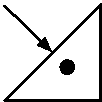
\includegraphics[scale=1]{images/mosterror.pdf}
\caption{The most erroneous spot in a right-angled simplex.}
\label{fig:mosterror}
\end{figure}

The error is presented as an ``average worst-case scenario".
The area of the reverse mapping space that is be the most erroneous is typically be the one furthest from the knots (corners of the simplex).
An illustration of this point is presented in Figure \ref{fig:mosterror}.
The point is halfway between all corners, except for the corner at the right angle.
This point is the most erroneous if the forward mapping is monotonically changing from one side of the simplex to the other (i.e., there are no local maxima or minima within the space).
Note that the reverse mapping will be identical to the forward mapping at the knots, since the forward mapping was used to infer their values.

Calculating the approximate upper bound on error, within a simplex, involves interpolating the system-level property value at the most erroneous point.
This is done by average the system-level property values of all corners not at the right angle.
Also, the location of the most erroneous point is queried for prediction through the forward mapping.
The difference between the interpolated value on the simplex and the actual predicted value using the forward mapping constitutes the error.
This metric is applied for every simplex and then averaged.
Thus, the metric measures the average error over all the worst-case scenarios for each simplex.
Also, the standard deviation of these errors is provided to convey how consistent the reverse mapping is.


  \subsubsection{Accuracy vs. Agent-Based Model Run}

The main goal of the reverse mapping is to be able to suggest configurations that would generate this behavior.
This approach is different from the previous metric because it measures the difference between the reverse mapping and the true behavior space.

\begin{figure}[ht]
\centering
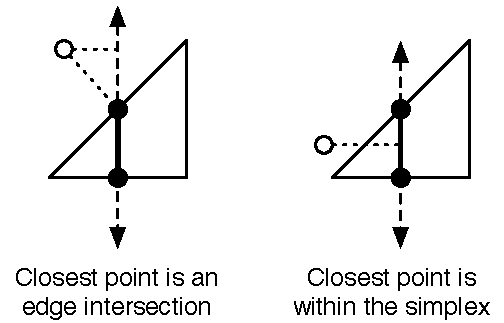
\includegraphics[scale=1]{images/closest.pdf}
\caption{Two cases for the closest point to a simplex intersection.}
\label{fig:closest}
\end{figure}

Error is measured by generating a random configuration point and sampling it from the agent-based model.
Then, the system-level property that was measured is passed to \fw to generate a reverse-mapping solution.
The error is the distance from the original configuration and the reverse-mapping solution space.
This value is calculated by adhering to the following procedure, per simplex:
\begin{enumerate}
  \item Determine the distance from the original point to the intersecting hyperplane.
  \item If the shortest line from the hyperplane to the point intersects the hyperplane \textit{within} the simplex, then the distance from the hyperplane is the distance from the intersection to the point.
  \item Otherwise, the closest point is one of the edge intersections.
\end{enumerate}
The two different cases (closest to an edge (left) and closest to the hyperplane (right)) are illustrated in Figure \ref{fig:closest}.
Then, the minimum from all these closest points is taken as the distance from the actual system-level property value and the value provided by the reverse mapping.
This distance is the error.

Several random configurations are sampled in this way.
The average and standard deviation of these errors are calculated to convey the accuracy of the reverse mapping, as well as the consistency of the reverse mapping.

  \subsubsection{Offline and Online Computation Time}
Offline computation time and online computation time is measured the same way for the reverse mapping as the forward mapping.
The amount of time \fw takes to prepare the reverse mapping is the offline computation time, and the amount of time required to produce a reverse mapping solution is the online computation time.



\section{Forward Mapping Methods}\label{sec:fmalgo}

\begin{itemize}
 \item k-Nearest Neighbor (KNN)
 \item Robust Locally Weighted Regression and Smoothing Scatterplots (LOESS)
 \item ?
\end{itemize}



\section{Experiments}\label{sec:exps}

 \subsection{Forward Mapping}

  \subsubsection{Accuracy}

  \subsubsection{Offline Computation Time}

  \subsubsection{Online Computation Time}

 \subsection{Reverse Mapping}

  \subsubsection{Accuracy vs. Forward Mapping}

  \subsubsection{Accuracy vs. System Run}

  \subsubsection{Offline Computation Time}

  \subsubsection{Online Computation Time}
